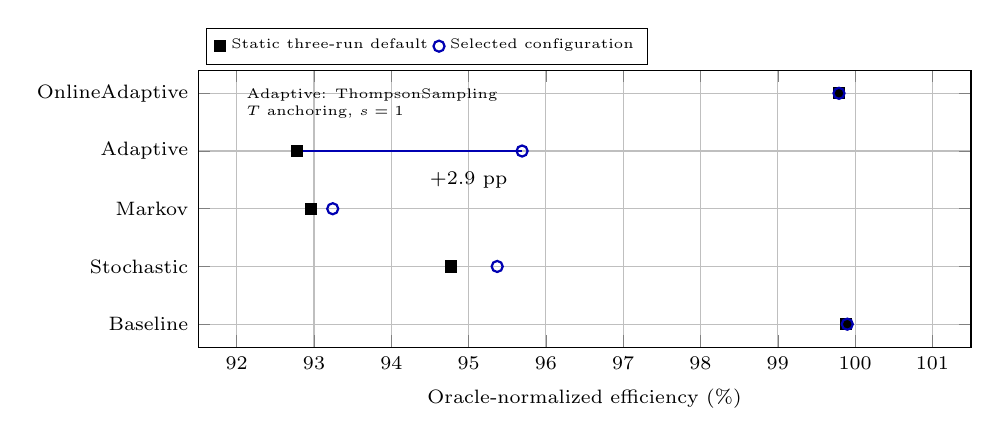
\begin{tikzpicture}
\begin{axis}[width=0.94\linewidth,height=5.1cm,xmin=91.5,xmax=101.5,
  xlabel={Oracle-normalized efficiency (\%)},ytick={0,1,2,3,4},
  yticklabels={Baseline,Stochastic,Markov,Adaptive,OnlineAdaptive},
  tick label style={font=\scriptsize},label style={font=\scriptsize},
  grid=major,legend style={font=\tiny,at={(0.01,1.02)},anchor=south west},
  legend columns=2]
\addplot[only marks,mark=square*,black] coordinates {(99.8851,0)(94.7703,1)(92.9563,2)(92.7833,3)(99.7923,4)};
\addlegendentry{Static three-run default}
\addplot[only marks,mark=o,blue!70!black,thick] coordinates {(99.899,0)(95.370,1)(93.242,2)(95.692,3)(99.792,4)};
\addlegendentry{Selected configuration}
\draw[blue!70!black] (axis cs:92.7833,3)--(axis cs:95.692,3);
\node[font=\scriptsize,anchor=north] at (axis cs:95,2.8) {$+2.9$ pp};
\node[font=\tiny,anchor=south west,align=left] at (axis cs:92,3.4) {Adaptive: ThompsonSampling\\$T$ anchoring, $s=1$};
\end{axis}
\end{tikzpicture}
